\section{Herramientas tecnológicas}
En esta sección presentaremos las herramientas tecnológicas estudiadas para el desarrollo de este trabajo. Se presenta un editor de ontologías llamado Protégé (ver \ref{subsection:protege}), un visualizador de ontologías en formato de grafo llamado VOWL (ver \ref{subsection:vowl}), un framework para la manipulación de datos en RDF, RDFS y OWL llamado Apache Jena (ver \ref{subsection:jena}) y una herramienta para realizar consultas SPARQL llamado Apache Jena Fuseki (ver \ref{subsection:fuseki}) .
\subsection{Protégé}
\label{subsection:protege}
Protégé es una herramienta de código libre para desarrolladores de ontologías y permite crear sistemas de base de conocimientos. El editor consiste en una interfaz gráfica de usuario donde podemos crear y editar clases, instancias, propiedades y restricciones. Nos permite guardar la ontología en varios formatos como XML, RDF, TTL y OWL. En la Figura \ref{img:protege} se muestra una captura de pantalla de la herramienta.

\begin{figure}[h!]
    \centering
    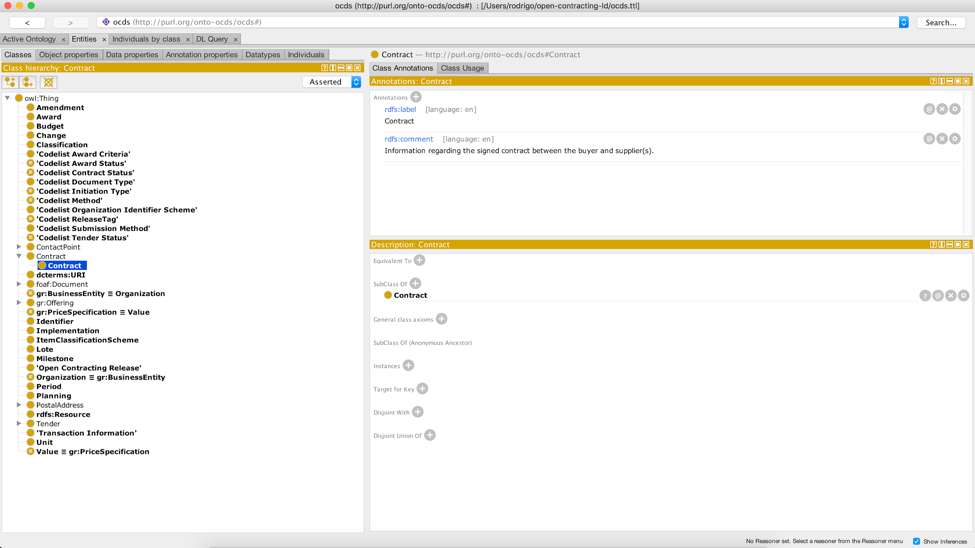
\includegraphics[width=150mm]{figuras/protege}
    \caption{Herramienta de Desarrollo de Ontologías: Protégé}
    \label{img:protege}
    \end{figure}

\subsection{Visual Notation for OWL}
\label{subsection:vowl}
Además se utilizó una herramienta de visualización gráfica de ontologías llamada \textit{Visual Notation for OWL} (VOWL) en su versión Web para visualizar de forma gráfica las ontologías estudiadas, en la Figura \ref{img:webvowl} se presenta una captura de pantalla de la herramienta utilizando como ejemplo una ontología llamada FOAF.

\begin{figure}[h!]
    \centering
    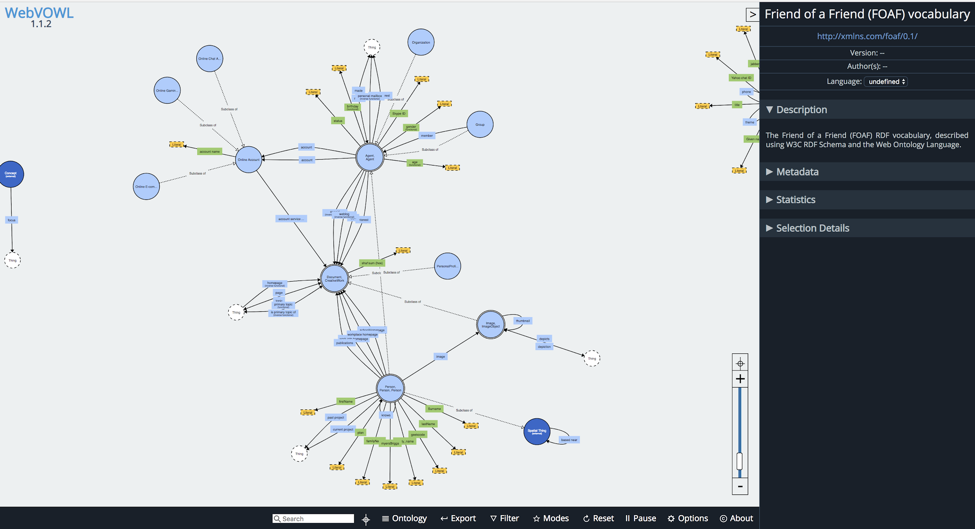
\includegraphics[width=150mm]{figuras/webvowl}
    \caption{Herramienta de Visualización de Ontologías: WebVOWL}
    \label{img:webvowl}
    \end{figure}
    

\subsection{Apache Jena}
\label{subsection:jena}
Jena es un \textit{Framework} implementado en JAVA para construir aplicaciones de la Web Semántica. Provee una librería para la manipulación de datos en RDF, RDFS, RDFa, OWL y SPARQL, y está alineada con las recomendaciones de la W3C. Jena incluye un motor de inferencias basado en reglas para realizar los razonamientos basados en OWL y RDFS, además de una variedad de estrategias para el almacenamiento de triplas RDF en memoria y en disco.

\subsection{Consulta de datos con SPARQL}
\label{subsection:fuseki}
Para consultar triplas basadas en RDF han surgido varios lenguajes de consulta, pero SPARQL es el más ampliamente utilizado y fue estandarizado por la W3C \cite{SPARQLDpoc:online}. Una consulta SPARQL es formulada usando patrones de grafos que pueden ser combinados con operaciones algebraicas como unión, opcional, filtro, etc. El resultado de la consulta es una lista de relaciones que pueden estar expresadas en tablas o en RDF.

A forma de explicar la semántica y sintaxis completa de este lenguaje, en el Cuadro \ref{lst:consulta-sparql} se muestra en un ejemplo la utilización del lenguaje realizando una consulta básica a la base de datos de DBPEDIA \cite{DBpedia:online} donde se listaron los nombres, fechas de nacimiento, fallecimiento y las URIs de personas nacidas en Paraguay antes de 1900, ordenadas por nombre.\hfill \break

\lstset{
    language=SPARQL, basicstyle=\linespread{0.8}\footnotesize\ttfamily
}
\noindent\begin{minipage}{\textwidth}
\begin{lstlisting}[captionpos=b, caption=Ejemplo de consulta SPARQL, label=lst:consulta-sparql,  numbers=left,  numberstyle=\tiny\color{mygray},frame=single]
PREFIX dbo: <http://dbpedia.org/ontology/>
PREFIX xsd: <http://www.w3.org/2001/XMLSchema#>
PREFIX foaf: <http://xmlns.com/foaf/0.1/>
PREFIX : <http://dbpedia.org/resource/>

SELECT ?name ?birth ?death ?person 
WHERE { 

    ?person dbo:birthPlace :Paraguay . 
    ?person dbo:birthDate ?birth . 
    ?person foaf:name ?name . 
    ?person dbo:deathDate ?death . 
    FILTER (?birth < "1900-01-01"^^xsd:date) . 
}
ORDER BY ?name
 
\end{lstlisting}
\end{minipage}

En las líneas 1 al 4 se pueden ver los prefijos de las ontologías utilizadas en la consulta, luego se presentan las triplas que componen las restricciones de la consulta. Está fuera del alcance de este documento la explicación detallada de la sintaxis de SPARQL.

Apache Jena Fuseki es un Servidor o Punto SPARQL que además provee un motor de inferencias. Se ejecuta como una aplicación web Java (archivo WAR). Provee el protocolo de consulta y actualización SPARQL 1.1 así como también el protocolo de \textit{SPARQL Graph Store}.
